\documentclass{article}
\usepackage[utf8]{inputenc}
\usepackage{array}
\usepackage{multicol}
\usepackage{listings}
\usepackage{amssymb}
\usepackage{enumitem}
\usepackage{graphicx}
\usepackage{amsthm}
\usepackage{hyperref}
\usepackage{tikz}
\usepackage{amssymb}
\usepackage{amsmath}
\usepackage{mathtools}

\begin{document}
\title{Functional Programming \\ Exercise set 4}
\date{\today}
\author{Tony Lopar s1013792 \\ Carlo Jessurun s1013793 \\ Marnix Dessing s1014097}
\maketitle

\section*{Exercise 1}
Most of these assignments are done in the ``BinaryTree.lhs''. However exercise 4.1.2 asks for visual representations so we've made those here:
\newline
\newline
\textbf{4.1.2}\\
\begin{center}
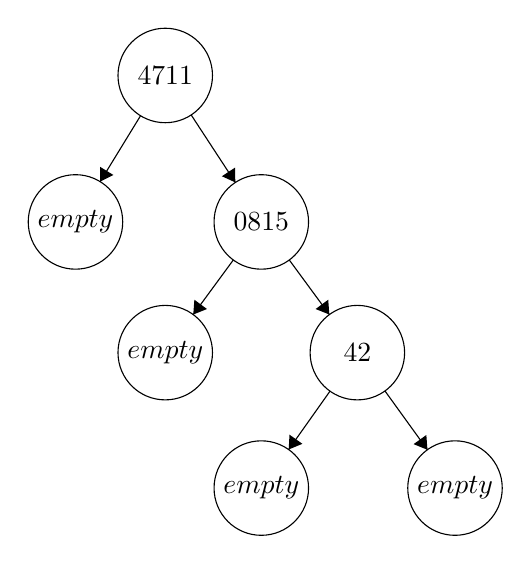
\begin{tikzpicture}[scale=0.2]
\tikzstyle{every node}+=[inner sep=0pt]
\draw [black] (36.8,-39) circle (3);
\draw (36.8,-39) node {$42$};
\draw [black] (43,-47.6) circle (3);
\draw (43,-47.6) node {$empty$};
\draw [black] (30.7,-47.6) circle (3);
\draw (30.7,-47.6) node {$empty$};
\draw [black] (30.7,-30.7) circle (3);
\draw (30.7,-30.7) node {$0815$};
\draw [black] (24.6,-39) circle (3);
\draw (24.6,-39) node {$empty$};
\draw [black] (24.6,-21.4) circle (3);
\draw (24.6,-21.4) node {$4711$};
\draw [black] (18.9,-30.7) circle (3);
\draw (18.9,-30.7) node {$empty$};
\draw [black] (38.55,-41.43) -- (41.25,-45.17);
\fill [black] (41.25,-45.17) -- (41.18,-44.23) -- (40.37,-44.81);
\draw [black] (35.06,-41.45) -- (32.44,-45.15);
\fill [black] (32.44,-45.15) -- (33.31,-44.79) -- (32.49,-44.21);
\draw [black] (32.48,-33.12) -- (35.02,-36.58);
\fill [black] (35.02,-36.58) -- (34.95,-35.64) -- (34.15,-36.23);
\draw [black] (28.92,-33.12) -- (26.38,-36.58);
\fill [black] (26.38,-36.58) -- (27.25,-36.23) -- (26.45,-35.64);
\draw [black] (26.25,-23.91) -- (29.05,-28.19);
\fill [black] (29.05,-28.19) -- (29.03,-27.25) -- (28.2,-27.8);
\draw [black] (23.03,-23.96) -- (20.47,-28.14);
\fill [black] (20.47,-28.14) -- (21.31,-27.72) -- (20.46,-27.2);
\end{tikzpicture}
\end{center}
\newpage
Second one:\\
\begin{center}
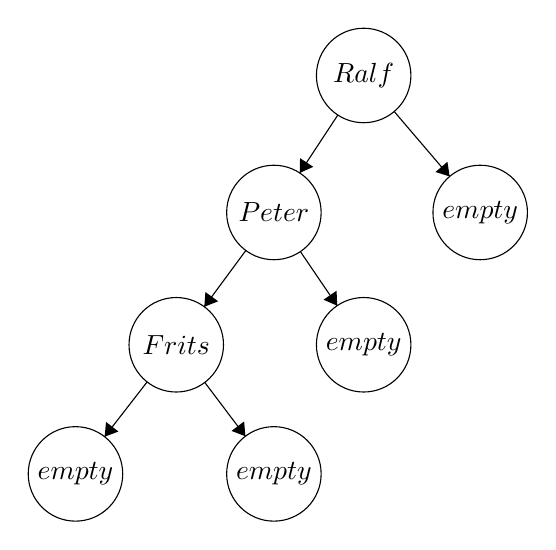
\begin{tikzpicture}[scale=0.2]
\tikzstyle{every node}+=[inner sep=0pt]
\draw [black] (38.7,-28.2) circle (3);
\draw (38.7,-28.2) node {$Ralf$};
\draw [black] (46.1,-36.9) circle (3);
\draw (46.1,-36.9) node {$empty$};
\draw [black] (33,-36.9) circle (3);
\draw (33,-36.9) node {$Peter$};
\draw [black] (38.7,-45.3) circle (3);
\draw (38.7,-45.3) node {$empty$};
\draw [black] (26.8,-45.3) circle (3);
\draw (26.8,-45.3) node {$Frits$};
\draw [black] (20.4,-53.5) circle (3);
\draw (20.4,-53.5) node {$empty$};
\draw [black] (33,-53.5) circle (3);
\draw (33,-53.5) node {$empty$};
\draw [black] (40.64,-30.49) -- (44.16,-34.61);
\fill [black] (44.16,-34.61) -- (44.02,-33.68) -- (43.26,-34.33);
\draw [black] (37.06,-30.71) -- (34.64,-34.39);
\fill [black] (34.64,-34.39) -- (35.5,-34) -- (34.66,-33.45);
\draw [black] (34.68,-39.38) -- (37.02,-42.82);
\fill [black] (37.02,-42.82) -- (36.98,-41.87) -- (36.15,-42.44);
\draw [black] (31.22,-39.31) -- (28.58,-42.89);
\fill [black] (28.58,-42.89) -- (29.46,-42.54) -- (28.65,-41.95);
\draw [black] (24.95,-47.66) -- (22.25,-51.14);
\fill [black] (22.25,-51.14) -- (23.13,-50.81) -- (22.34,-50.2);
\draw [black] (28.61,-47.69) -- (31.19,-51.11);
\fill [black] (31.19,-51.11) -- (31.11,-50.17) -- (30.31,-50.77);
\end{tikzpicture}
\end{center}
Third one:\\
\begin{center}
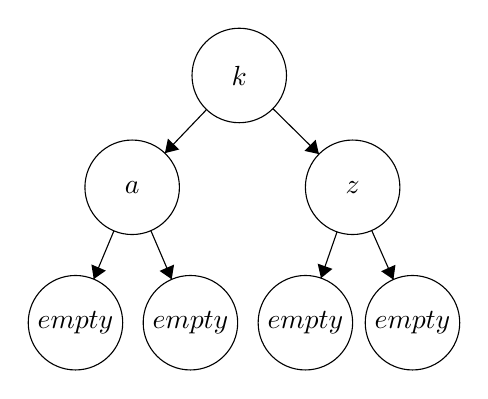
\begin{tikzpicture}[scale=0.2]
\tikzstyle{every node}+=[inner sep=0pt]
\draw [black] (37.9,-44) circle (3);
\draw (37.9,-44) node {$empty$};
\draw [black] (23.3,-44) circle (3);
\draw (23.3,-44) node {$empty$};
\draw [black] (30.6,-44) circle (3);
\draw (30.6,-44) node {$empty$};
\draw [black] (33.7,-28.3) circle (3);
\draw (33.7,-28.3) node {$k$};
\draw [black] (26.9,-35.4) circle (3);
\draw (26.9,-35.4) node {$a$};
\draw [black] (40.9,-35.4) circle (3);
\draw (40.9,-35.4) node {$z$};
\draw [black] (44.7,-44) circle (3);
\draw (44.7,-44) node {$empty$};
\draw [black] (31.62,-30.47) -- (28.98,-33.23);
\fill [black] (28.98,-33.23) -- (29.89,-33) -- (29.17,-32.31);
\draw [black] (35.84,-30.41) -- (38.76,-33.29);
\fill [black] (38.76,-33.29) -- (38.55,-32.38) -- (37.84,-33.09);
\draw [black] (25.74,-38.17) -- (24.46,-41.23);
\fill [black] (24.46,-41.23) -- (25.23,-40.69) -- (24.31,-40.3);
\draw [black] (28.09,-38.16) -- (29.41,-41.24);
\fill [black] (29.41,-41.24) -- (29.56,-40.31) -- (28.64,-40.71);
\draw [black] (39.91,-38.23) -- (38.89,-41.17);
\fill [black] (38.89,-41.17) -- (39.62,-40.58) -- (38.68,-40.25);
\draw [black] (42.11,-38.14) -- (43.49,-41.26);
\fill [black] (43.49,-41.26) -- (43.62,-40.32) -- (42.71,-40.73);
\end{tikzpicture}
\end{center}
\textbf{4.1.5}
The depth of a node is the number of edges from the node to the tree's root node.
A root node will have a depth of 0.
The height of a node is the number of edges on the longest path from the node to a leaf.
A leaf node will have a height of 0. Therefore there is no real relation between these numbers. The size of the tree is usually can often be equal to the maxheight if the given tree is balanced. Given the above examples however, this is not the case.
\section*{Exercise 2}


\section*{Exercise 3}


\section*{Exercise 4}
\begin{enumerate}
  \item The difference between the function member that's defined in exercise 4.1.6 is that this function doesn't need to check both children of the node if the value is unequal to the value of the node. When the value is less we only need to check the left child and if it's greater only the right child.
  \item The function is implemented in BinarySearchTree.lhs. It checks the node and recursively inserts the value left if it's smaller or equal and right if it's greater.
  \item If an element that is a leave is deleted, then we simply may return Empty for the subtree. Otherwise we should replace it with the greatest lower element or the lowest greater element.
  \item The function should check whether the left child is lower or equal and whtether the right child is greater or equal. It should also check whether this also holds for the children of both childs. If one of the children is Empty only the other one should be checked.
\end{enumerate}

\section*{Exercise 5}
\begin{enumerate}
  \item
\end{enumerate}

\section*{Exercise 6}



\end{document}
